% !TEX root = ../arbeit.tex
\chapter{Evaluation}\label{chapter:evaluation}
To validate the fineness and quality of the proposed PROCAMS a technical evaluation was executed. In particular, the precision and speed of the pan-tilt unit were examined as well as the touch accuracy. Finally, overall performance of the PROCAMS is evaluated.
While planning the execution of larger usability studies in a domestic environment this evaluation should give a first clue of strengths and weaknesses of the build PROCAMS. 

\section{Pan-Tilt Unit Performance}
The task of the pan-tilt unit is to move the PROCAMS fast and accurate to a desired location. This two properties accuracy and pace were assessed in a laboratory study.

\subsection{Alignment Accuracy}
The accuracy approaching a previously stored position was determined by placing the PROCAMS with a distance of \SI{1}{\m} to a wall. The projector was displaying a red cross to indicate the centre of the projection. Then the pan-tilt unit was commanded to approach the stored position from eight defined starting points. The position where the red cross came to a standstill was marked at the wall.
Starting points were up, up-right, right, right-down, down, down-left, left, and left-up. Where up and down indicates a vertical shift by \SI{45}{\degree} from the stored position. Accordingly left and right indicates a horizontal shift by \SI{90}{\degree}. The measured distances in horizontal a vertical direction between the marked and stored position lead to an angel of aberration by simple trigonometry.
The stored position was approached ten times from each starting point. Thus 80 data points were obtained. A plot of the data is shown in~\autoref{plot:movement}.
% !TEX root = ../arbeit.tex
\begin{figure}[htbp]
        \centering
\tikzset{mark options={mark size=2, line width=1.5pt}}
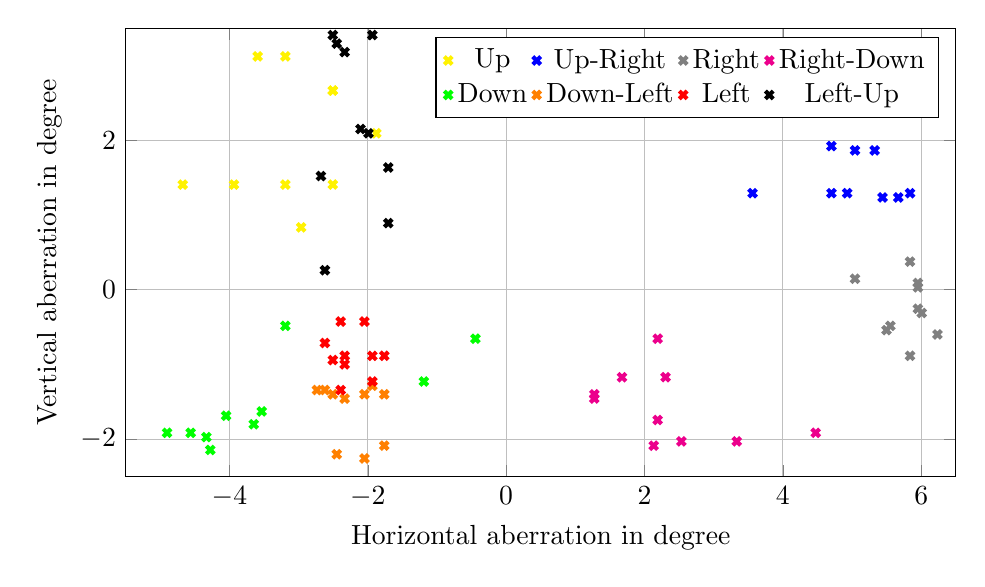
\begin{tikzpicture}
	\begin{axis}[%
	width=\textwidth,
	height = .6\textwidth,
	xmax = 6.5,
	xmin = -5.5,
	xstep= 1,
	ymin = -2.5,
	ymax =3.5,
	ystep=1,
	grid=major,
	legend columns=4,
	xlabel=Horizontal aberration in degree,
	ylabel=Vertical aberration in degree,
	scatter/classes={
		Up={mark=x,yellow},
		Up-Right={mark=x,blue},
		Right={mark=x,gray},
		Right-Down={mark=x,magenta},
		Down={mark=x,green},
		Down-Left={mark=x,orange},
		Left={mark=x,red},
		Left-Up={mark=x,black}
		}]
	\addplot[scatter,only marks,%
		scatter src=explicit symbolic]%
	table[meta=label] {
x     y      label
-4.67424872612533	1.40704466542326			Up
-3.93360909963853	1.40704466542326			Up
-3.1916505442666	1.40704466542326			Up
-2.9631282497019	0.834310816061917			Up
-2.50580769586769	1.40704466542326			Up
-1.87648177481699	2.09394419785448			Up
-2.50580769586769	2.66590922345048			Up
-3.59131574999252	3.12310419675389			Up
-3.1916505442666	3.12310419675389			Up
-2.50580769586769	2.66590922345048			Up
4.87197278490512	3.12310419675389			Up-Right
4.70128244616578	1.922268042484			Up-Right
5.04257648050957	1.8650348309974			Up-Right
5.32671540617036	1.8650348309974			Up-Right
5.44029823293142	1.23524883003786			Up-Right
5.66733440279074	1.23524883003786			Up-Right
5.83749482341844	1.29251672941418			Up-Right
4.70128244616578	1.29251672941418			Up-Right
4.92885045666407	1.29251672941418			Up-Right
3.56135251033059	1.29251672941418			Up-Right
5.83749482341844	-0.8844333423724			Right
5.49707362345356	-0.5407128664187			Right
5.55383818745301	-0.483421668036623			Right
6.23412919364215	-0.598002983536637			Right
5.950877911401	-0.254248352762198			Right
6.00755197509656	-0.311542730726946			Right
5.950877911401	0.0322288725769704			Right
5.950877911401	0.0895245826339467			Right
5.83749482341844	0.375998155486819			Right
5.04257648050957	0.146820113642666			Right
2.13256625938215	-2.08679175426757			Right-Down
3.33299828852148	-2.02956988177023			Right-Down
2.18978055419555	-1.74340203526284			Right-Down
1.27390493988743	-1.39988698938846			Right-Down
1.27390493988743	-1.45714715525241			Right-Down
1.67470826450442	-1.17081949820428			Right-Down
2.30419592354254	-1.17081949820428			Right-Down
2.18978055419555	-0.655291904866927			Right-Down
4.47356567736875	-1.9151140985677			Right-Down
2.53297060324095	-2.02956988177023			Right-Down
-4.90183476990765	-1.9151140985677			Down
-4.56039979299942	-1.9151140985677			Down
-4.33259451138178	-1.9723439586187			Down
-4.27562145717918	-2.14400946240445			Down
-3.64838313294688	-1.80064302302008			Down
-3.53424123132033	-1.62890972945458			Down
-3.1916505442666	-0.483421668036623			Down
-1.18943272767241	-1.22809016670015			Down
-0.444749555610536	-0.655291904866927			Down
-4.0476456276837	-1.68615756608216			Down
-2.44861895803739	-2.20122289252437			Down-Left
-2.04816744014753	-2.25843193102194			Down-Left
-1.76200574367305	-2.08679175426757			Down-Left
-2.7345115584368	-1.34262402653776			Down-Left
-2.62017007131273	-1.34262402653776			Down-Left
-2.50580769586769	-1.39988698938846			Down-Left
-2.33422694871262	-1.45714715525241			Down-Left
-2.04816744014753	-1.39988698938846			Down-Left
-1.76200574367305	-1.39988698938846			Down-Left
-1.93371422794441	-1.28535838089828			Down-Left
-2.62017007131273	-0.712579515900411			Left
-2.50580769586769	-0.941714567461968			Left
-2.33422694871262	-0.8844333423724			Left
-1.93371422794441	-0.8844333423724			Left
-1.76200574367305	-0.8844333423724			Left
-2.39142533786276	-1.34262402653776			Left
-1.93371422794441	-1.22809016670015			Left
-2.39142533786276	-0.426129502926883			Left
-2.04816744014753	-0.426129502926883			Left
-2.33422694871262	-0.998993909972118			Left
-2.62017007131273	0.261410180165005			Left-Up
-1.70476239345517	0.891593594551635			Left-Up
-2.67734348248654	1.5215613564293			Left-Up
-1.70476239345517	1.6360658892936			Left-Up
-1.99094282098346	2.09394419785448			Left-Up
-2.1053879716975	2.15116137745379			Left-Up
-2.33422694871262	3.1802267828006			Left-Up
-2.44861895803739	3.29445285887791			Left-Up
-2.50580769586769	3.40865272433571			Left-Up
-1.93371422794441	3.40865272433571			Left-Up
	};

\addlegendentry{Up}
\addlegendentry{Up-Right}
\addlegendentry{Right}
\addlegendentry{Right-Down}
\addlegendentry{Down}
\addlegendentry{Down-Left}
\addlegendentry{Left}
\addlegendentry{Left-Up}

	\end{axis}
\end{tikzpicture}
\caption{Aberration of the pan-tilt unit approaching a defined location}
\label{plot:movement}
\end{figure}

The average horizontal misalignment is \SI{3,29}{\degree}. For vertical alignment, the average error is \SI{1,48}{\degree}. Hence, the misalignment in an arbitrary direction is \SI{3,74}{\degree}. This accords to a shift of less than \SI{10}{\cm} if the \emph{surface} is \SI{150}{\cm} away from the projector.
A likely reason for the smaller misalignment in the vertical direction is caused by an additionally used accelerometer to control the servo for horizontal alignment. Since, for horizontal alignment no secondary sensor is used, the alignment is not as good. Overall the alignment is fair enough to re-project a widget at almost the same location in the physical world, but is not sufficient enough to augment small tangible objects as for example a light switch. 

A more accurate alignment could be achieved by two different modifications. On the one hand, a sensor providing very accurate data for horizontal and vertical alignment could be attached to provide feedback of the current alignment of the pan-tilt unit. Nonetheless, previous attempts already showed that a simple calibrated and compensated compass is not suitable for this task since the projector and servos have a strong influence on the magnetic field.

On the other hand, more powerful servos with a high resolution potentiometer could be installed. The potentiometer would lead the servo to move more precisely to the commanded position. This approach seems very promising without any major change at the pan-tilt unit. 

\subsection{Alignment Pace}
The pace of the pan-tilt unit was evaluated in a separate benchmark. Therefor, the time needed for \SI{164}{\degree} horizontal pan and a \SI{110}{\degree} tilt was measured. Each movement was repeated ten times from both directions. Since panning and tilting is performed simultaneously no combinations of tilt and pan were executed.

On average the pan-tilt unit needed \SI{3.5}{\second} for the horizontal pan task. For the tilt task, the unit needed \SI{4.8}{\second}. A reason for the slower tilt movement could be the higher force needed for tilting compared to the rotation force. Overall the PROCAMS can reach every position in less than \SI{6}{\second} (worst-case: move \SI{135}{\degree} vertically). This seems to be a decent time.
Of course, there are faster servos available, but higher acceleration forces could damage the printed case holding the PROCAMS. 


\section{Touch Performance}
Touch performance was evaluated in a basic laboratory study. The PROCAMS was mounted over a desk in a distance of \SI{75}{\cm}. It was tilted down \SI{70}{\degree} from horizontal, pointing at the desk illuminating an \textit{interaction space} of \SI{40 x 30}{\cm}. The setup is shown in~\autoref{img:evalSetup}. Four red crosses surround by a white circle posed as target. They were distributed on three different \textit{surfaces}. Two targets at the desk, one at the cardboard box on the left side and one on a ramp composed of a red notebook. The four targets are depicted in~\autoref{img:evalTargets}. In all cases, the diameter of the red cross was \SI{18}{\mm}.
\begin{figure}
        \centering
        \begin{subfigure}[b]{0.31\textwidth}
                \includegraphics[width=\textwidth]{images/evaluation/targets.png}
                \caption{Four target positions for touch evaluation}
                \label{img:evalTargets}
        \end{subfigure}
	\hfill         
        \begin{subfigure}[b]{0.31\textwidth}
                \includegraphics[width=\textwidth]{images/evaluation/setup.png}
                \caption{Evaluation setup: PROCAMS and touch targets }
                \label{img:evalSetup}
        \end{subfigure}
	\hfill          
        \begin{subfigure}[b]{0.31\textwidth}      
                \includegraphics[width=\textwidth]{images/evaluation/touch.png}
                \caption{Green border indicates a detected touch}
                \label{img:EvalTouchDetection}
        \end{subfigure}
        \caption{Touch accuracy evaluation setup}
        \label{fig:TouchEval}
\end{figure}

During the study participants had the task to touch the targets as accurately as possible. Participants were ordered to take as much time as needed. Forty targets were presented in a counterbalanced order, one at a time. A detected touch was indicated by a green border (see~\autoref{img:EvalTouchDetection}). After touching the target, it disappeared and appeared at one of the three other positions.
Time as well as touch position in projector and world coordinate system were monitored. From that data, the error in mm in the world coordinate system can be derived.  

Ten participants between 24 and 27 years took part in this study. Hence, 400 touch events were monitored. On average participants needed \SI{109}{\second} to touch all 40 target. In less than 1\% the touch was not detected on the first approach. This was counted manually. Distribution of monitored touch events for each target is shown in \autoref{fig:touchperformance}. The targets are labeled as follows: cardboard box (T1), ramp (T2), left desk(T3) and right desk (T4). 
\input{chapters/plotTouch}

Collected touch data was analysed with a standard weighted-means ANOVA test (F=57.06, p<0.0001)  in conjunction with a  Tukey's honest significance test.
The mean touch error, variance and standard deviation for the different targets is specified in~\autoref{tab:touchErrorEval}.

In this study setup, T1 has a significantly smaller error than T2, T3 and T4 (p<0.01, HSD[.01]=1.3). This coincides with \textcite{Hardy:2012jo} results, who identify that the accuracy of touch detection mainly depends on sensor distance. Target 1 was closest to the camera. The significantly worse result of T2 in comparison to T3 and T4 (p<0.01, HSD[.01]=1.3) cannot be explained by distance since it was very similar. A likely reason could be the material and colour of the notebook, but further investigations are necessary. 

\begin{table}[htb]
\begin{tabularx}{\textwidth}{ l|XXXl}
\toprule
Target & T1 & T2 & T3 & T4 \\
\midrule
Mean (in mm) & 14.1104 & 19.3232 & 16.5835 & 17.82 \\
Variance & 8.4757 & 12.4966 & 8.5013 & 7.5729 \\
Std. deviation (in mm) & 2.9113 & 3.5351 & 2.9157 & 2.7519 \\
Significant versus & T2,T3,T4 & T3,T4 \\
\bottomrule
\end{tabularx}
\caption{Statistical data}
\label{tab:touchErrorEval}
\end{table}

A mean error of less than \SI{20}{\mm} requires large buttons for pleasant interaction. However, the small standard deviation for all targets is remarkable. It appears that for the evaluation setup a fixed offset between executed and detected touch was present. It is necessary to figure out how and where this offset emerged and if the offset could be correct. 
The offset could accrue at several positions in the processing pipeline. First of all a bad calibration file between the projector and camera could lead to errors. Although, this is unlikely since a new calibration file was created before the evaluation. A likely reason for non optimal detection could be the different field of views of projector and depth sensing camera. The projected image fills only an area of approximately \SI{340x220}{px} which is roughly $\sfrac{1}{4}$ of the available resolution. To improve this issue a projector with a short throw lens or a camera with zoom lens should be used to adapt the field of views. Finally, a non-conform transformation matrix could result in the error. A source code recheck could clarify this concern.

\subsection{Touch Pace}
Even though the depth sensing camera runs at 30 \ac{fps} on average only 21.8 fps are processed. In particular, processing limitations and the Qt event-queue are responsible for that loss of frames. Due to the used tracking users must press a target for at least three frames which is equivalent to \SI{0.138}{\second}. In the study it was only problematic for the first one or two targets since participants know instant detection from their smart phones. After explaining to interact slightly slower participants could interact in an enjoyable way. 


\section{Overall Performance}
Overall, the proposed PROCAMS performs well. Widgets are rendered with up to 30 fps.
As mentioned before, touch detection runs at almost 22 fps. This performance remains also when two to three individual widgets are added to different \textit{surfaces}. Adding more widgets will decrease the available processing power and touch detection slows down to 10 to 14 fps. This forces the user to interact in an unnatural slow way. For more synchronous rendered content alternative rendering techniques or more processing power are required. 

\section{Conclusion}
To assess the quality and performance of the build PROCAMS an evaluation was conducted. Pan-tilt unit and touch detection were analysed in separate studies. The pan-tilt unit fulfils the requirements and can approach a stored position in a short space of time. However, accuracy of the servos could be more accurate. Numerous possibilities of improvement were discussed.

Touch detection accuracy is very reasonable with a small standard deviation of less than \SI{3.5}{\mm}. Touch accuracy is comparable to other PROCAMS requiring a manual calibration task. Enabling touch detection on arbitrary surfaces without any setup specific calibration was a tough task. Mapping of detected touch points back to the projection makes is even more prone to failure. From this point of view and considering inexpensive hardware the touch accuracy is very auspicious.